\begin{surferPage}[Singularidad A3+-]{Una singularidad $A_3^{+-}$}
Su ecuación, $x^4+y^2-z^2=0$, es similar a la de $A_2^{+-}$, $x^3+y^2-z^2$,
con la diferencia de que es también simétrica respecto del plano $yz$, ya
que
    \[(-x)^4+y^2-z^2=x^4+y^2-z^2.\]
Es, pues, simétrica respecto de los tres planos de coordenadas, pues
$y\mapsto -y$ (respectivamente $z\mapsto -z$) no cambia la ecuación.

Como para la taza de café, podemos ver una singularidad
$A_3^{+-}$ cuando la luz solar atraviesa un vaso de te:
    \vspace*{0.5ex}
    \begin{center}
      \begin{tabular}{c@{\qquad}c}
        \begin{tabular}{@{}c@{}}
          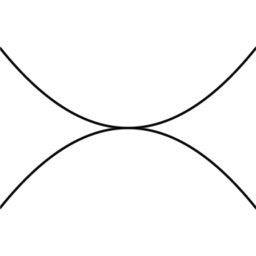
\includegraphics[width=1.4cm]{../../common/images/A3pm_cut_rot}
        \end{tabular}
        &
        \begin{tabular}{@{}c@{}}
          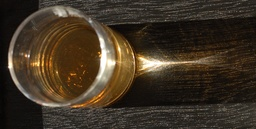
\includegraphics[height=1.4cm]{../../common/images/teeglas_detail}
        \end{tabular}
      \end{tabular}
    \end{center}
    \vspace*{0ex}
La deformación en dos singularidades cónicas (que es posible según
se ha explicado en el texto de la singularidad $A_2^{+-}$),
tiene el siguiente aspecto:
    %
    \begin{center}
      \begin{tabular}{@{}c@{\quad}c@{\quad}c@{}}
        \begin{tabular}{@{}c@{}}
          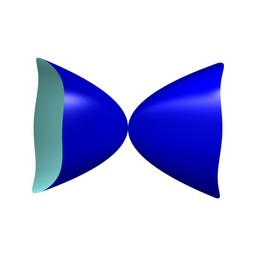
\includegraphics[width=1.2cm]{../../common/images/A3pm_0}
        \end{tabular}
        &
        \begin{tabular}{@{}c@{}}
          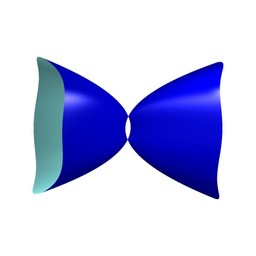
\includegraphics[width=1.2cm]{../../common/images/A3pm_1}
        \end{tabular}
        &
        \begin{tabular}{@{}c@{}}
          
\includegraphics[width=1.2cm]{../../common/images/A3pm_2}
        \end{tabular}
      \end{tabular}
    \end{center}
 
\end{surferPage}
